% "Станет проще"

\documentclass[a4paper,12pt]{article} % тип документа

% report, book

% Рисунки
\usepackage{graphicx}
\usepackage{wrapfig}
\usepackage{lscape}

\usepackage{hyperref}
\usepackage[rgb]{xcolor}
\hypersetup{				% Гиперссылки
    colorlinks=true,       	% false: ссылки в рамках
	urlcolor=blue          % на URL
}

%  Русский язык

\usepackage[T2A]{fontenc}			% кодировка
\usepackage[utf8]{inputenc}			% кодировка исходного текста
\usepackage[english,russian]{babel}	% локализация и переносы


% Математика
\usepackage{amsmath,amsfonts,amssymb,amsthm,mathtools} 
\DeclarePairedDelimiter\abs{\lvert}{\rvert}%


\usepackage{wasysym}

%Заговолок
\author{Поляченко Юрий \\ 726}
\title{Уравнения мелкой воды}
\date{\today}

\begin{document} % начало документа

\clearpage\maketitle
\thispagestyle{empty}

\newpage

\tableofcontents

\newpage

\section{Аналитический анализ}

Решается система уравнений

\begin{equation} \label{eq:anal_vecForm}
\begin{aligned}
&\frac{\partial \vec{V}}{\partial t}=-g \nabla h\\
&\frac{\partial h}{\partial t}+\bar{H}(\nabla \cdot \vec{V})=0
\end{aligned} .
\end{equation}

Работаем в 2D, что физически соответствует например воде в бассейне $\Omega = [0; L_x] \times [0; L_y]$. Покомпонентно система запишется как

\begin{equation}
\begin{aligned}
&\frac{\partial u}{\partial t}=-g \frac{\partial h}{\partial x}\\
&\frac{\partial v}{\partial t}=-g \frac{\partial h}{\partial y}\\
&\frac{\partial h}{\partial t}+H\left(\frac{\partial u}{\partial x}+\frac{\partial v}{\partial y}\right)=0
\end{aligned}.
\end{equation}

Для простоты численных оценок в реальных расчетах будем считать g = H = 1, если не оговорено иного.

Для получения аналитических решений удобно избавиться от <<не наблюдаемых>> переменных $u$ и $v$. \eqref{eq:anal_vecForm} приводится к волновому уравнению.

\begin{equation}
\ddot{h}(t, \vec{x}) = g H \cdot \Delta h(t, \vec{x}).
\end{equation}

Граничные условия непротекания

\begin{equation}
\begin{aligned}
& u(x = 0) = u(x = L_x) = 0 \\
& v(y = 0) = v(y = L_y) = 0 \\
\end{aligned},
\end{equation}

естественные для задачи воды в бассейне, приводят к условиям на $h$:

\begin{equation}
\begin{aligned}
& h'_x(x = 0) = h'_x(x = L_x) = 0 \\
& h'_y(y = 0) = h'_y(y = L_y) = 0 \\
\end{aligned}.
\end{equation}

Или, короче и общее

\begin{equation}
\left. \dfrac{dh}{d \vec{n}} \right|_{\partial \Omega} = 0
\end{equation}

Все вышесказанное позволяет нам выписать общее решение задачи:

\begin{equation}
\begin{cases}
&\frac{\partial u}{\partial t}=-g \frac{\partial h}{\partial x}\\
&\frac{\partial v}{\partial t}=-g \frac{\partial h}{\partial y}\\
&\frac{\partial h}{\partial t}+H\left(\frac{\partial u}{\partial x}+\frac{\partial v}{\partial y}\right)=0 \\
& h'_x(x = 0) = h'_x(x = L_x) = 0 \\
& h'_y(y = 0) = h'_y(y = L_y) = 0 \\
& h(t = 0, x, y) = f(x, y) \\
& u(t = 0, x, y) = u_0(x, y) \\
& v(t = 0, x, y) = v_0(x, y) \\
\end{cases}
\end{equation}

приводит к

\begin{equation}
\begin{aligned}
& k_{xn} = \dfrac{\pi}{L_x} \left( n + \dfrac{1}{2} \right), \hspace{10pt} k_{ym} = \dfrac{\pi}{L_y} \left( m + \dfrac{1}{2} \right), \hspace{10pt} n,m \in \mathbb{N} \\
& e_{nm}(x,y) = \cos{(x k_{xn})} \cos{(y k_{ym})} \sqrt{\dfrac{2}{L_x}} \sqrt{\dfrac{2}{L_y}} \\
& \omega_{nm}^2 = g H (k_{xn}^2 + k_{ym}^2) \\
& w(x,y) = -H \left( \dfrac{\partial u_0}{\partial x} + \dfrac{\partial v_0}{\partial y} \right) \\
& w_{nm} = (w, e_{nm}), \hspace{10pt} f_{nm} = (f, e_{nm}) \\
& g_{nm}(t) = \dfrac{w_{nm}}{\omega_{nm}} \sin{(\omega_{nm} t)} + f_{nm} \cos{(\omega_{nm} t)} \\
& h(t, x, y) = \sum_{n, m} g_{nm}(t) e_{nm}(x,y). \\
\end{aligned}
\end{equation}

Где введено 

\begin{equation}
(f,g) = \int\limits_0^{L_y} \int\limits_0^{L_x} f(x,y) g(x,y) dx dy.
\end{equation}

Для ПГУ решения выглядят аналогично, только базисные функции немного отличаются

\begin{equation}
\begin{aligned}
& e_{nm}(x,y) = e_n(x) e_m(y)  \\
& e_n(x) = 
\begin{cases}
\cos{\left( x \dfrac{\pi n}{L_x} \right)} \sqrt{\dfrac{2}{L_x}}, \hspace{10pt} n \mathrel{\vdots} 2 \\ 
\sin{\left( x \dfrac{\pi (n+1)}{L_x} \right)} \sqrt{\dfrac{2}{L_x}}, \hspace{10pt} n \not{\mathrel{\vdots}} \hspace{3pt} 2 \\
\end{cases} \\
\end{aligned}
\end{equation}

Например если взять начальные уловия 

\begin{equation}
\begin{aligned}
& h(t = 0, x, y) = \cos{\left( x \dfrac{2 \pi}{L_x} \right)} + \cos{\left( 2 y \dfrac{2 \pi}{L_y} \right)} \\
& u(t = 0) = 0, \hspace{10pt} v(t = 0) = 0, \\
\end{aligned}
\end{equation}

то решение как для ПГУ так и для непротекания будет

\begin{equation}
h(t, x, y) = \cos{\left( x \dfrac{2 \pi}{L_x} \right)} \cos{\left( t \dfrac{2 \pi v_0}{L_x} \right)} + \cos{\left( 2 y \dfrac{2 \pi}{L_y} \right)} \cos{\left( 2 t \dfrac{2 \pi v_0}{L_y} \right)},
\end{equation}

где $v_0^2 = g H$.

\newpage

\section{Численное решение на А-сетке}

\subsection{Анализ апрокcимации и устойчивости}
... - надо ли?

\subsection{Численные эксперименты}

Для первых тестов были реализованы симметричные схемы 2 порядка по времени и пространству. 1-ый шаг по времени делался обычным Эйлером. Проведена проверка порядка схемы - при изменении шага $dx$ по пространству и выборе $dt = dx/3v_0$ для устойчивости MSD отклонения от точного решения. Ожидаемый результат $(sup_{\tau < t}[\delta^2(\tau)])(t) < (\mathcal{O}(dt^3) * T/dt)^2 = \mathcal{O}(dt^4 T^2) \sim dt^4$

\begin{figure}[h!]
\begin{center}
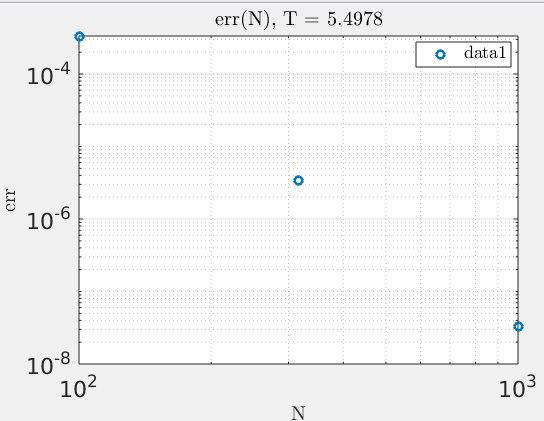
\includegraphics[width=0.6\textwidth]{./pics/Atype_nErr}
\end{center}
\caption{Зависимость среднего (по пространству) квадрата отклонения численного решения от точного при $dt = dx/3v_0$ и $T = T_{period} \cdot 7/8$. При этом физическом времени расчета проходится максимум ошибки, поэтому на нем корректно сравнивать схему при разных шагах интегрирования. Шаги уменьшились на 1 порядок, а $\delta^2$ уменьшилась на 4 порядка, т.е. $\delta$ линейно уменьшилаь на 2 - все сходится.} \label{img:Atype_nErr}
\end{figure}

\newpage

По графику роста ошибки от времени виден порядок роста $(sup_{\tau < t}[\delta^2(\tau)])(t) < \mathcal{O}(dt^4 T^2) \sim T^2$

\begin{figure}[h!]
\begin{center}
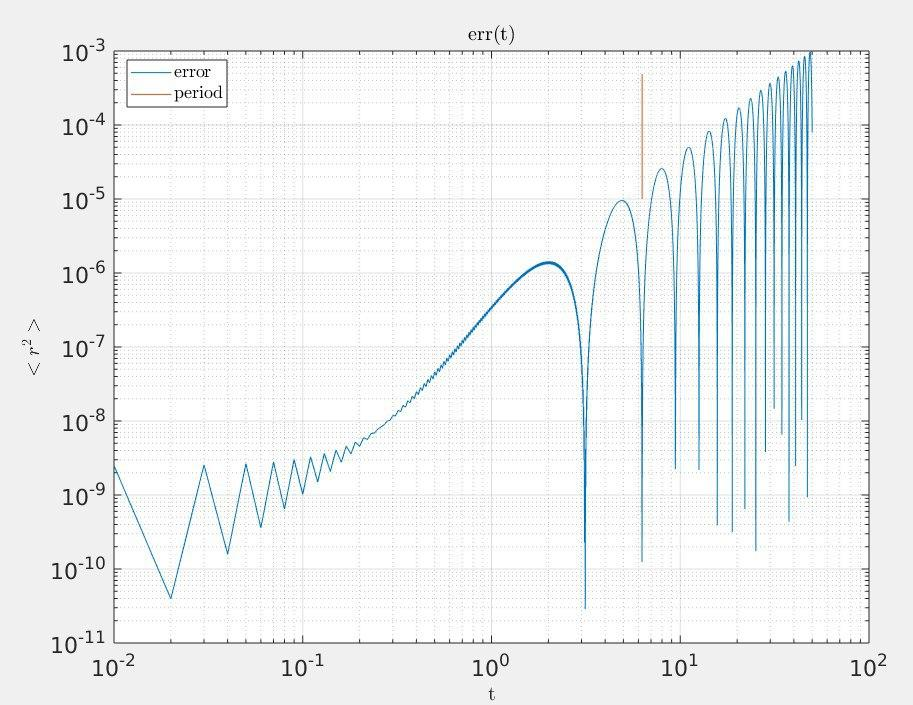
\includegraphics[width=0.85\textwidth]{./pics/Atype_tErr}
\end{center}
\caption{Зависимость среднего квадрата отклонения численного решения от точного. Устанавливается рост $\sim t^2$, что и ожидалось.} \label{img:Atype_tErr}
\end{figure}

\subsection{Дополнительные моменты}

\begin{itemize}
\item В процессе отладки была встречена проблема $2h$ - грамоники, являющейся следствием применения центральной расности для 1-ой производной. Если взять волну с $\lambda = 2 \delta x$, то в узлах сетки будут значения $h_{nm} = (-1)^{m+n}$, откуда 

\begin{equation}
\begin{aligned}
& \dot{u} = \dfrac{-1 - (-1)}{2 \delta x} = 0 \\
& \dot{v} = \dfrac{-1 - (-1)}{2 \delta y} = 0 \\
\end{aligned}
\end{equation}

\end{itemize}

\newpage

\section{Численное решение на C-сетке}

\subsection{Анализ апрокcимации и устойчивости}
... - надо ли?

\subsection{Численные эксперименты}

\subsubsection{Центральная разность}

В А-сетках значения всех определяемых функций известны на одном наборе точек $(t,x,y)_{ijk}$. На С-сетках для уравнений мелкой воды наборы точек по пространству для $u$, $v$ и $h$ отличаются. Для начала была реализована симметричная расность 2 порядка точности, для которой ошибка схемы ведет себя ожидаемо

\begin{figure}[h!]
\begin{center}
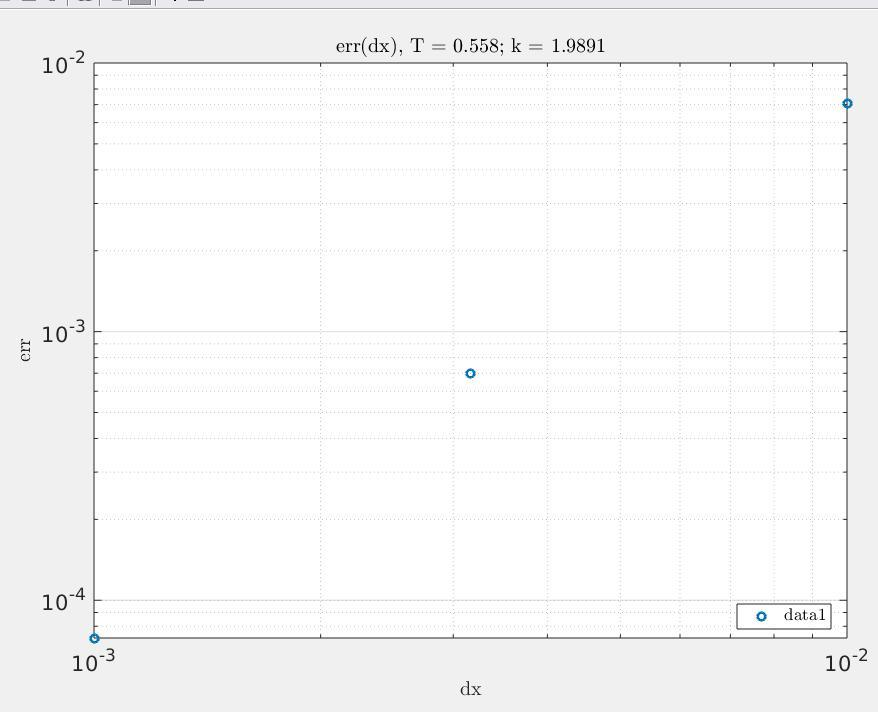
\includegraphics[width=0.7\textwidth]{./pics/Ctype_nErr}
\end{center}
\caption{Зависимость среднего (по пространству) квадрата отклонения численного решения от точного при $dt = dx/3v_0$ и $T = T_{period} \cdot 7/8$. При этом физическом времени расчета проходится максимум ошибки, поэтому на нем корректно сравнивать схему при разных шагах интегрирования. Шаги уменьшились на 1 порядок, а $\delta$ линейно уменьшилась на 2 - все сходится.} \label{img:Atype_nErr}
\end{figure}

\end{document} % конец документа